\appendix
\section{Technical appendix}
\label{sec:appendix}

\subsection{Pen portraits of the British Spatial Signature types}
\label{sec:appendixD}

\begin{longtable}{p{0.25\textwidth}p{0.7\textwidth}}
    \caption{\label{tab:pens}Interpretative pen portraits characterising each signature type based on its numerical profile. Reproduced from \cite{fleischmann2022geographical} published under CC-BY 4.0.}\\

    \toprule
    Signature type &                                                                                                                                                                                                                                                                                                                                                                                                                             Pen Portait \\
    \midrule
    \endfirsthead

    \toprule
    Signature type &                                                                                                                                                                                                                                                                                                                                                                                                                             Pen Portait \\
    \midrule
    \endhead
    \midrule
    \multicolumn{2}{r}{{Continued on next page}} \\
    \midrule
    \endfoot

    \bottomrule
    \endlastfoot

    Wild countryside                     &                                                                                       In “Wild countryside”, human influence is the least intensive. This signature covers large open spaces in the countryside where no urbanisation happens apart from occasional roads, cottages, and pastures. You can find it across the Scottish Highlands, numerous national parks such as Lake District, or in the majority of Wales. \\
    Countryside agriculture              &                                                                                                                                                                               “Countryside agriculture” features much of the English countryside and displays a high degree of agriculture including both fields and pastures. There are a few buildings scattered across the area but, for the most part, it is green space. \\
    Urban buffer                         &                                                                                             “Urban buffer” can be characterised as a green belt around cities. This signature includes mostly agricultural land in the immediate adjacency of towns and cities, often including edge development. It still feels more like countryside than urban, but these signatures are much smaller compared to other countryside types. \\
    Open sprawl                          &                                                                                                                           “Open sprawl” represents the transition between countryside and urbanised land. It is located in the outskirts of cities or around smaller towns and is typically made up of large open space areas intertwined with different kinds of human development, from highways to smaller neighbourhoods. \\
    Disconnected suburbia                &                                                                                                                                           “Disconnected suburbia” includes residential developments in the outskirts of cities or even towns and villages with convoluted, disconnected street networks, low built-up and population densities, and lack of jobs and services. This signature type is entirely car-dependent. \\
    Accessible suburbia                  &                                        “Accessible suburbia” covers residential development on the urban periphery with a relatively legible and connected street network, albeit less so than other more urban signature types. Areas in this signature feature low density, both in terms of population and built-up area, lack of jobs and services. For these reasons, “accessible suburbia” largely acts as dormitories. \\
    Warehouse/Park land                  &                                “Warehouse/Park land” covers predominantly industrial areas and other work-related developments made of box-like buildings with large footprints. It contains many jobs of manual nature such as manufacturing or construction, and very little population live here compared to the rest of urban areas. Occasionally this type also covers areas of parks with large scale green open areas. \\
    Gridded residential quarters         &                                                                                  “Gridded residential quarters” are areas with street networks forming a well-connected grid-like (high density of 4-way intersections) pattern, resulting in places with smaller blocks and higher granularity. This signature is mostly residential but includes some services and jobs, and it tends to be located away from city centres. \\
    Connected residential neighbourhoods &                                                                     “Connected residential neighbourhoods” are relatively dense urban areas, both in terms of population and built-up area, that tend to be formed around well-connected street networks. They have access to services and some jobs but may be further away from city centres leading to higher dependency on cars and public transport for their residents. \\
    Dense residential neighbourhoods     &                                                                                                                                           A “dense residential neighbourhood” is an abundant signature often covering large parts of cities outside of their centres. It has primarily residential purpose and high population density, varied street network patterns, and some services and jobs but not in high intensity. \\
    Dense urban neighbourhoods           &                                                                                                                            “Dense urban neighbourhoods” are areas of inner-city with high population and built-up density of a predominantly residential nature but with direct access to jobs and services. This signature type tends to be relatively walkable and, in the case of some towns, may even form their centres. \\
    Local urbanity                       &                                                                “Local urbanity” reflects town centres, outer parts of city centres or even district centres. In all cases, this signature is very much urban in essence, combining high population and built-up density, access to amenities and jobs. Yet, it is on the lower end of the hierarchy of signature types denoting urban centres with only a local significance. \\
    Regional urbanity                    &                                                             “Regional urbanity” captures centres of mid-size cities with regional importance such as Liverpool, Plymouth or Newcastle upon Tyne. It is often encircled by “Local urbanity” signatures and can form outer rings of city centres in large cities. It features high population density, as well as a high number of jobs and amenities within walkable distance. \\
    Metropolitan urbanity                &                                                                                    Signature type “Metropolitan urbanity” captures the centre of the largest cities in Great Britain such as Glasgow, Birmingham or Manchester. It is characterised by a very high number of jobs in the area, high built-up density and often high population density. This type serves as the core centre of the entire metropolitan areas. \\
    Concentrated urbanity                &  Concentrated urbanity” is a signature type found in the city centre of London and nowhere else in Great Britain. It reflects the uniqueness of London in the British context with an extremely high number of jobs and amenities located nearby, as well as high built-up and population densities. Buildings in this signature are large and tightly packed, forming complex shapes with courtyards and little green space. \\
    Hyper concentrated urbanity          &     The epitome of urbanity in the British context. “Hyper concentrated urbanity” is a signature type present only in the centre of London, around the Soho district, and covering Oxford and Regent streets. This signature is the result of centuries of urban primacy, with a multitude of historical layers interwoven, very high built-up and population density, and extreme abundance of amenities, services and jobs. \\
    \bottomrule
\end{longtable}


\subsection{Method of data splitting}
\label{sec:appendixF}

Due to the potential data leakage caused by pixels shared by chips present in both
train and validation sets, we have developed a method of spatial data splitting that
ensures no data leakage happens. While this could be done randomly, such a subdivision
does not allow for sliding, the splits are required to be spatially contiguous. The
method therefore proceeds as follows:

\begin{enumerate}
    \item Create a grid of chips of a set size covering the entire study area.
    \item Eliminate chips that are not fully within a single signature geometry.
    \item Sort chips using the space-filling Hilbert curve.
    \item Subdivide chips within each contiguous signature geometry into four parts:
    40\% for CNN training, 10\% for CNN validation, 40\% for probability modelling
    training, 10\% for probability modelling validation. This subdivision is node based
    on the Hilbert distance ensuring spatial compactness and contiguity of each part.
    For signature geometries that are too small to be subdivided, the entire geometry is
    used within one set only.
    \item (If SIC) Apply sliding within each part.
\end{enumerate}


\subsection{Comparison of neural network architecture}
\label{sec:appendixA}

\begin{table}[H]
    \centering
\begin{tabular}{llll}
    \toprule
    architecture & top layer & \# neurons in top layer &       global accuracy \\
    \midrule
    EfficientNetB4 &   Flatten &                    128 &  0.663482 \\
    EfficientNetB4 &   Flatten &                    256 &  0.715764 \\
    EfficientNetB4 &   Flatten &                    512 &  0.697187 \\
    EfficientNetB4 &   GlobalAveragePooling2D &                    128 &  0.723726 \\
    EfficientNetB4 &   GlobalAveragePooling2D &                    256 &  0.715764 \\
    EfficientNetB4 &   GlobalAveragePooling2D &                    512 &  0.727972 \\
        ResnNet50 &   Flatten &                    128 &  0.481157 \\
        ResnNet50 &   Flatten &                    256 &  0.481423 \\
        ResnNet50 &   Flatten &                    512 &  0.522824 \\
        ResnNet50 &   GlobalAveragePooling2D &                    128 &  0.469745 \\
        ResnNet50 &   GlobalAveragePooling2D &                    256 &  0.469745 \\
        ResnNet50 &   GlobalAveragePooling2D &                    512 &  0.526274 \\
           VGG19 &   Flatten &                    128 &  0.708333 \\
           VGG19 &   Flatten &                    256 &  0.675425 \\
           VGG19 &   Flatten &                    512 &  0.692144 \\
           VGG19 &   GlobalAveragePooling2D &                    128 &   0.69931 \\
           VGG19 &   GlobalAveragePooling2D &                    256 &  0.678609 \\
           VGG19 &   GlobalAveragePooling2D &                    512 &   0.67224 \\
    \bottomrule
    \end{tabular}
\caption{\label{tab:app_nns}\footnotesize Comparison of global accuracy of different
architectures of neural network on a sample of data with signature types aggregated into
three classes (centres, periphery, countryside) using the baseline image classification.
EfficientNetB4 with GlobalAveragePooling2D and 256 neurons has been used in the final
experiment.}
\end{table}


\pagebreak

\subsection{Within-class performance by spatial signature}
\label{sec:appendixB}

\begin{figure}
    \centering
    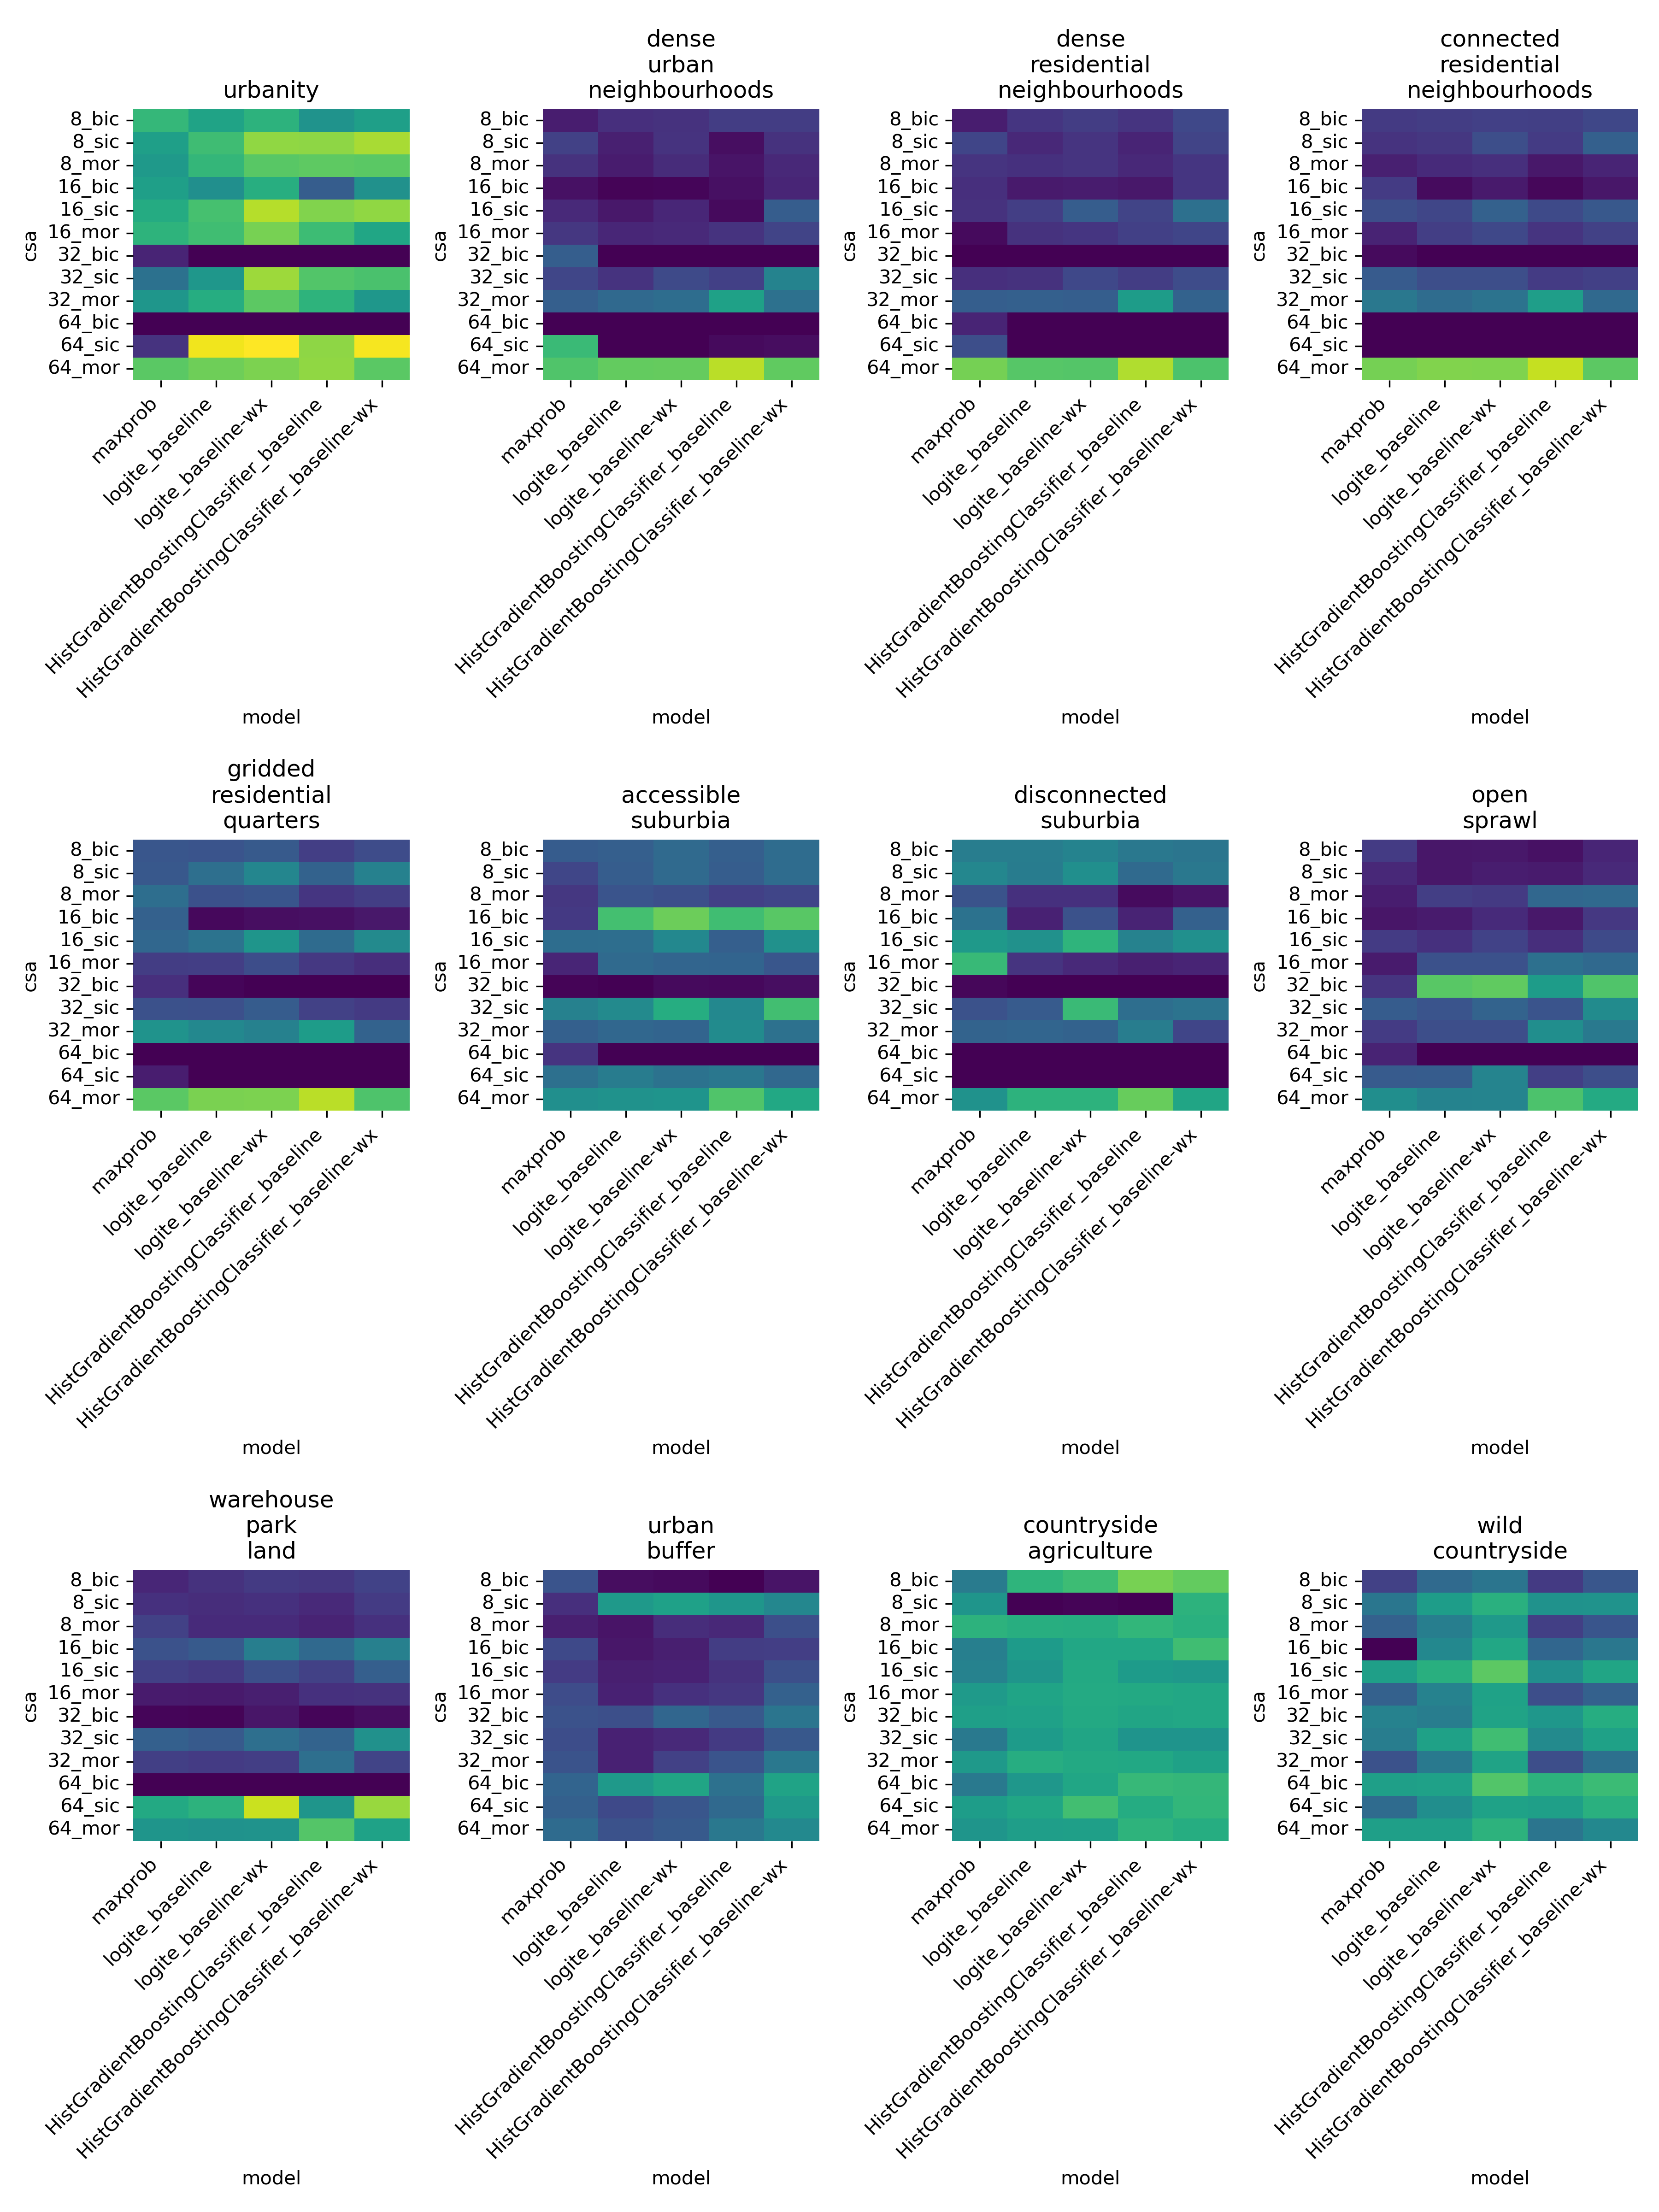
\includegraphics[width=0.8\linewidth]{fig/wc_accuracy_x_signature.png}
    \caption{\footnotesize Within-class accuracy scores grouped by signature. Each panel
    represents results from one of the 12 signatures predicted. Each column in
    the heatmap
    corresponds to one of the five models compared, namely:
    histogram-based boosted classifier (\texttt{HGBC}) with features
    pertaining only to a given chip (\texttt{baseline}) or including also features
    from neighbouring ones (\texttt{baseline-wx}); Logit ensemble
    (\texttt{logite}) with the same two variations; and a simpler maximum
    probability approach (\texttt{maxprob}). Each row
    corresponds to a pair of chipsize (8, 16, 32, and 64 pixels)
    and architecture (baseline image classification, or \texttt{bic}; sliding
            image classification, or \texttt{sic}; and multi-output
    regression, or \texttt{mor}) used in the neural network stage of the
    pipeline.}
    \label{fig:wc_accuracy_x_signature}
\end{figure}

\pagebreak

\subsection{Confusion matrices}
\label{sec:appendixC}

\begin{figure}
    \centering
    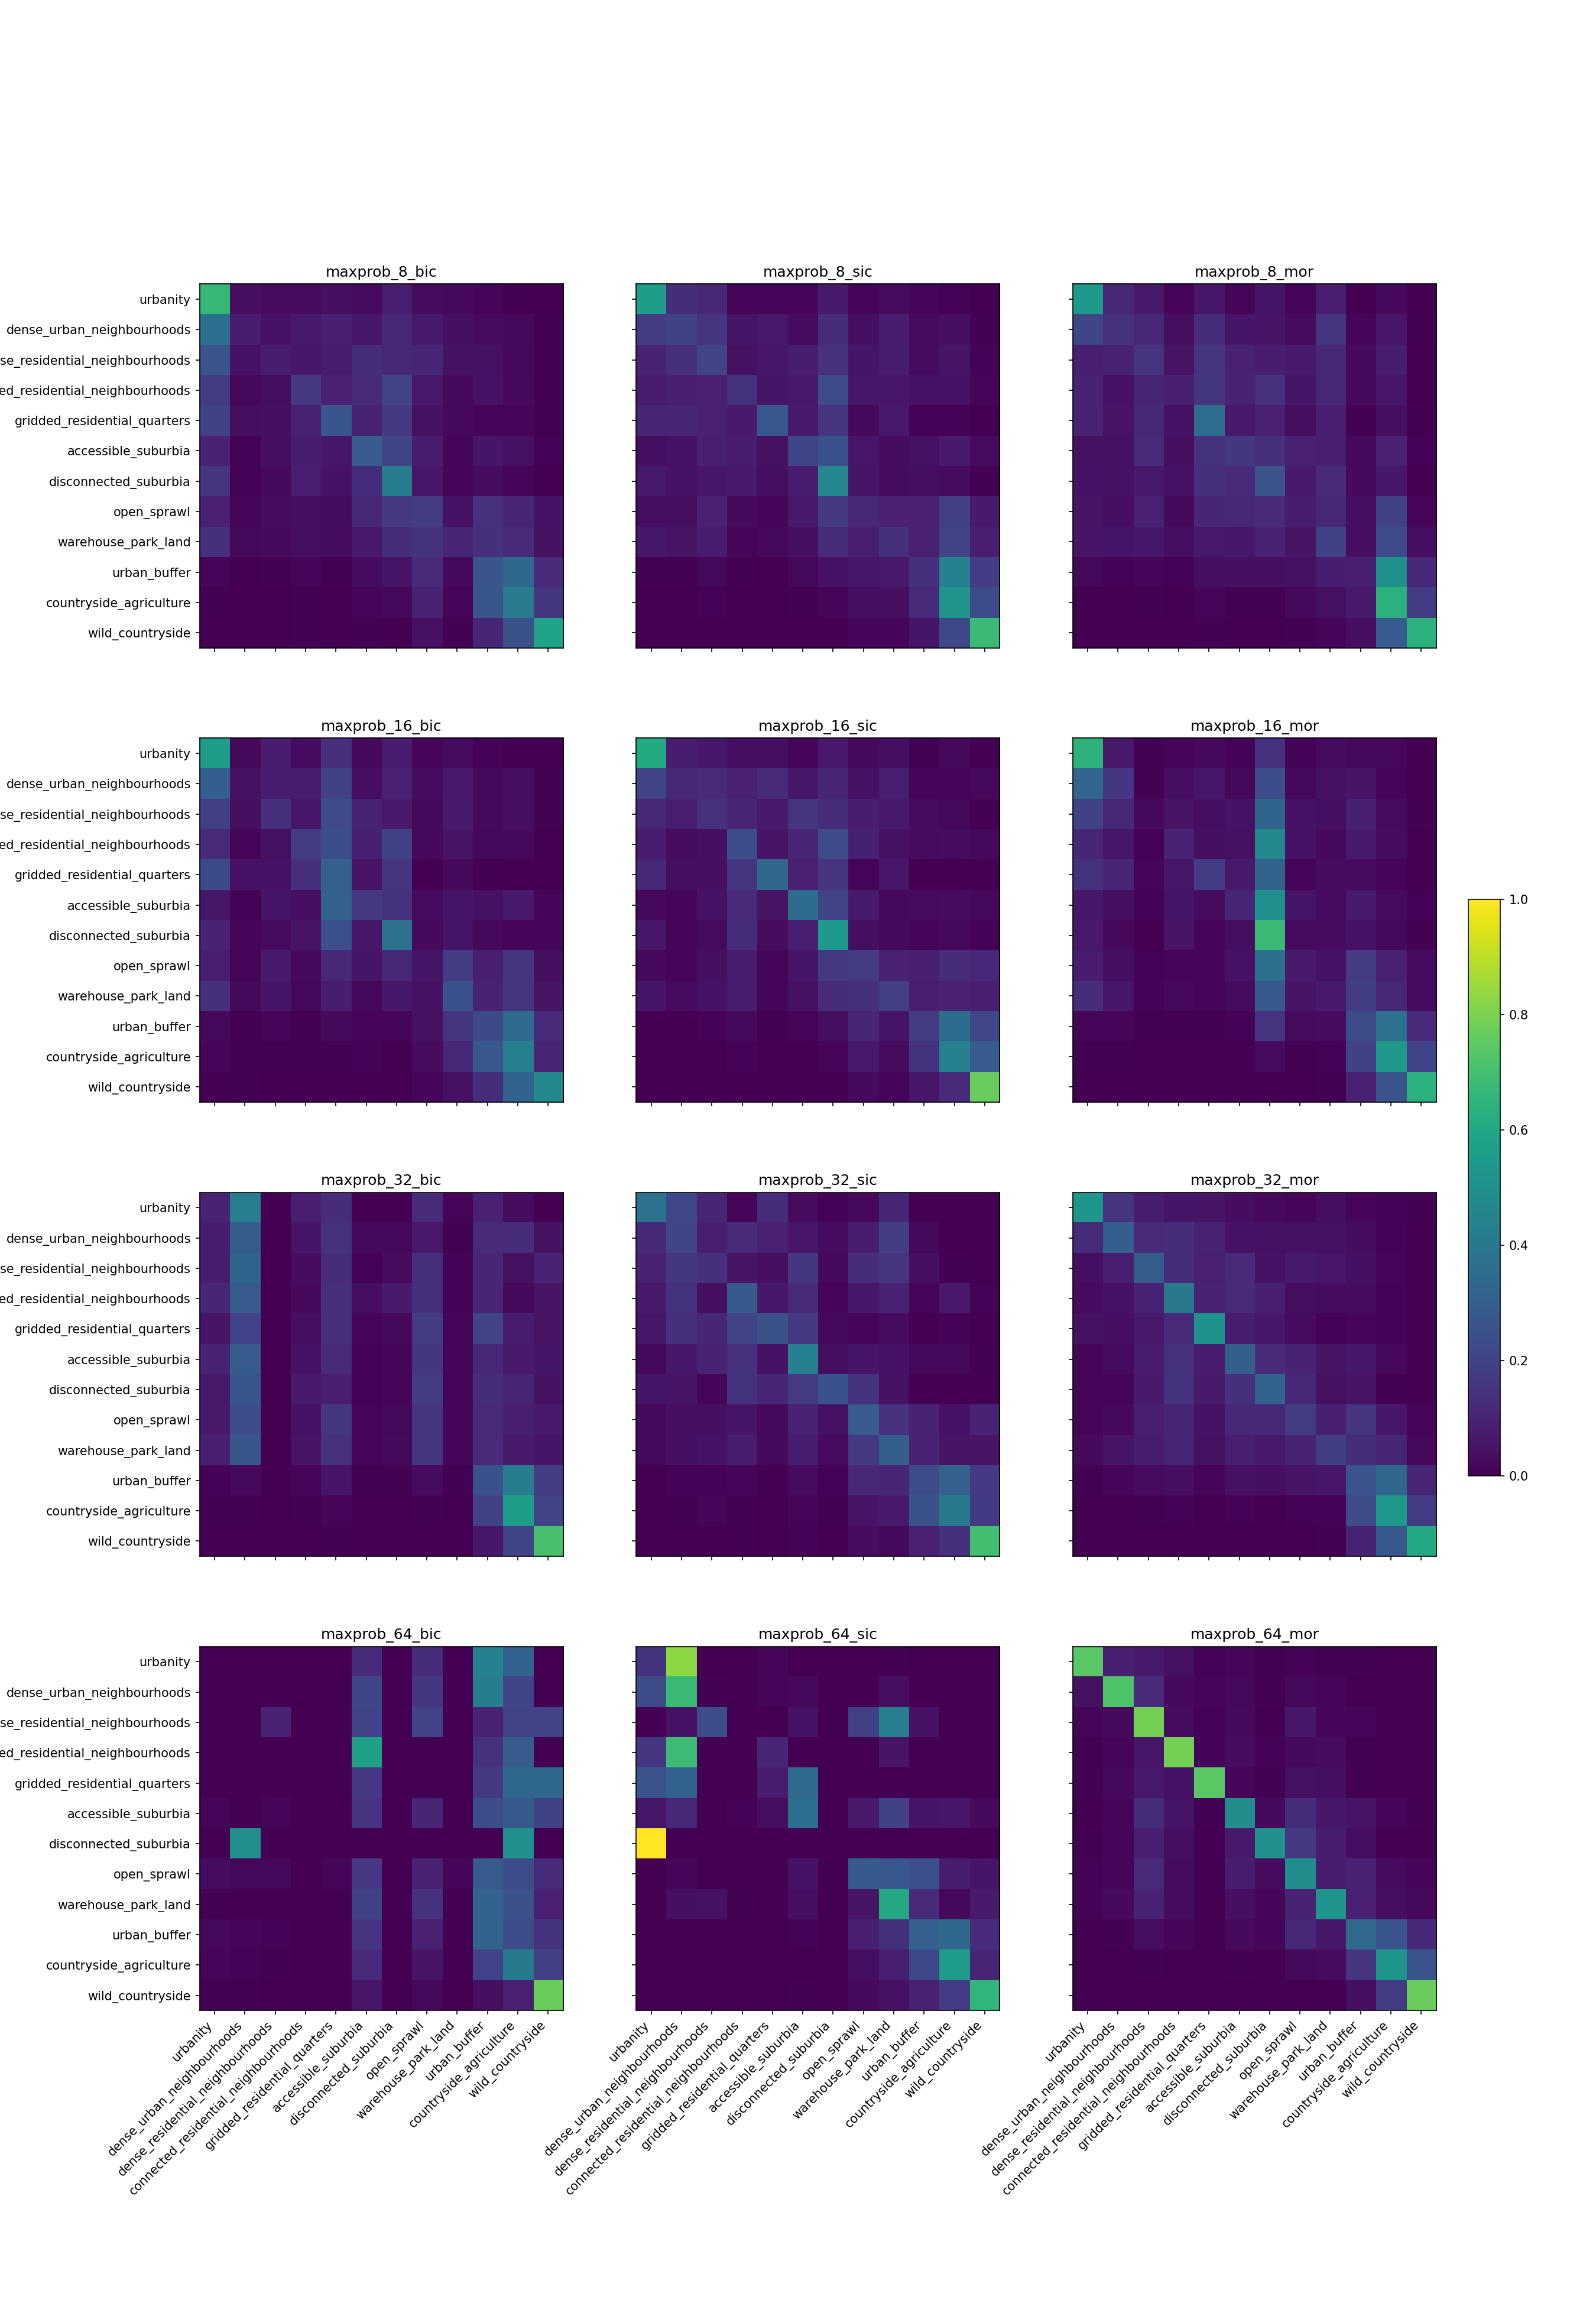
\includegraphics[width=.9\linewidth]{fig/maxprob_cm.png}
    \caption{\footnotesize Confusion matrices for individual models denoting
    the ability of each model in prediction of a correct label per each class
    using the maximum probability architecture.}
    \label{fig:maxprob_cm}
\end{figure}


\begin{figure}
    \centering
    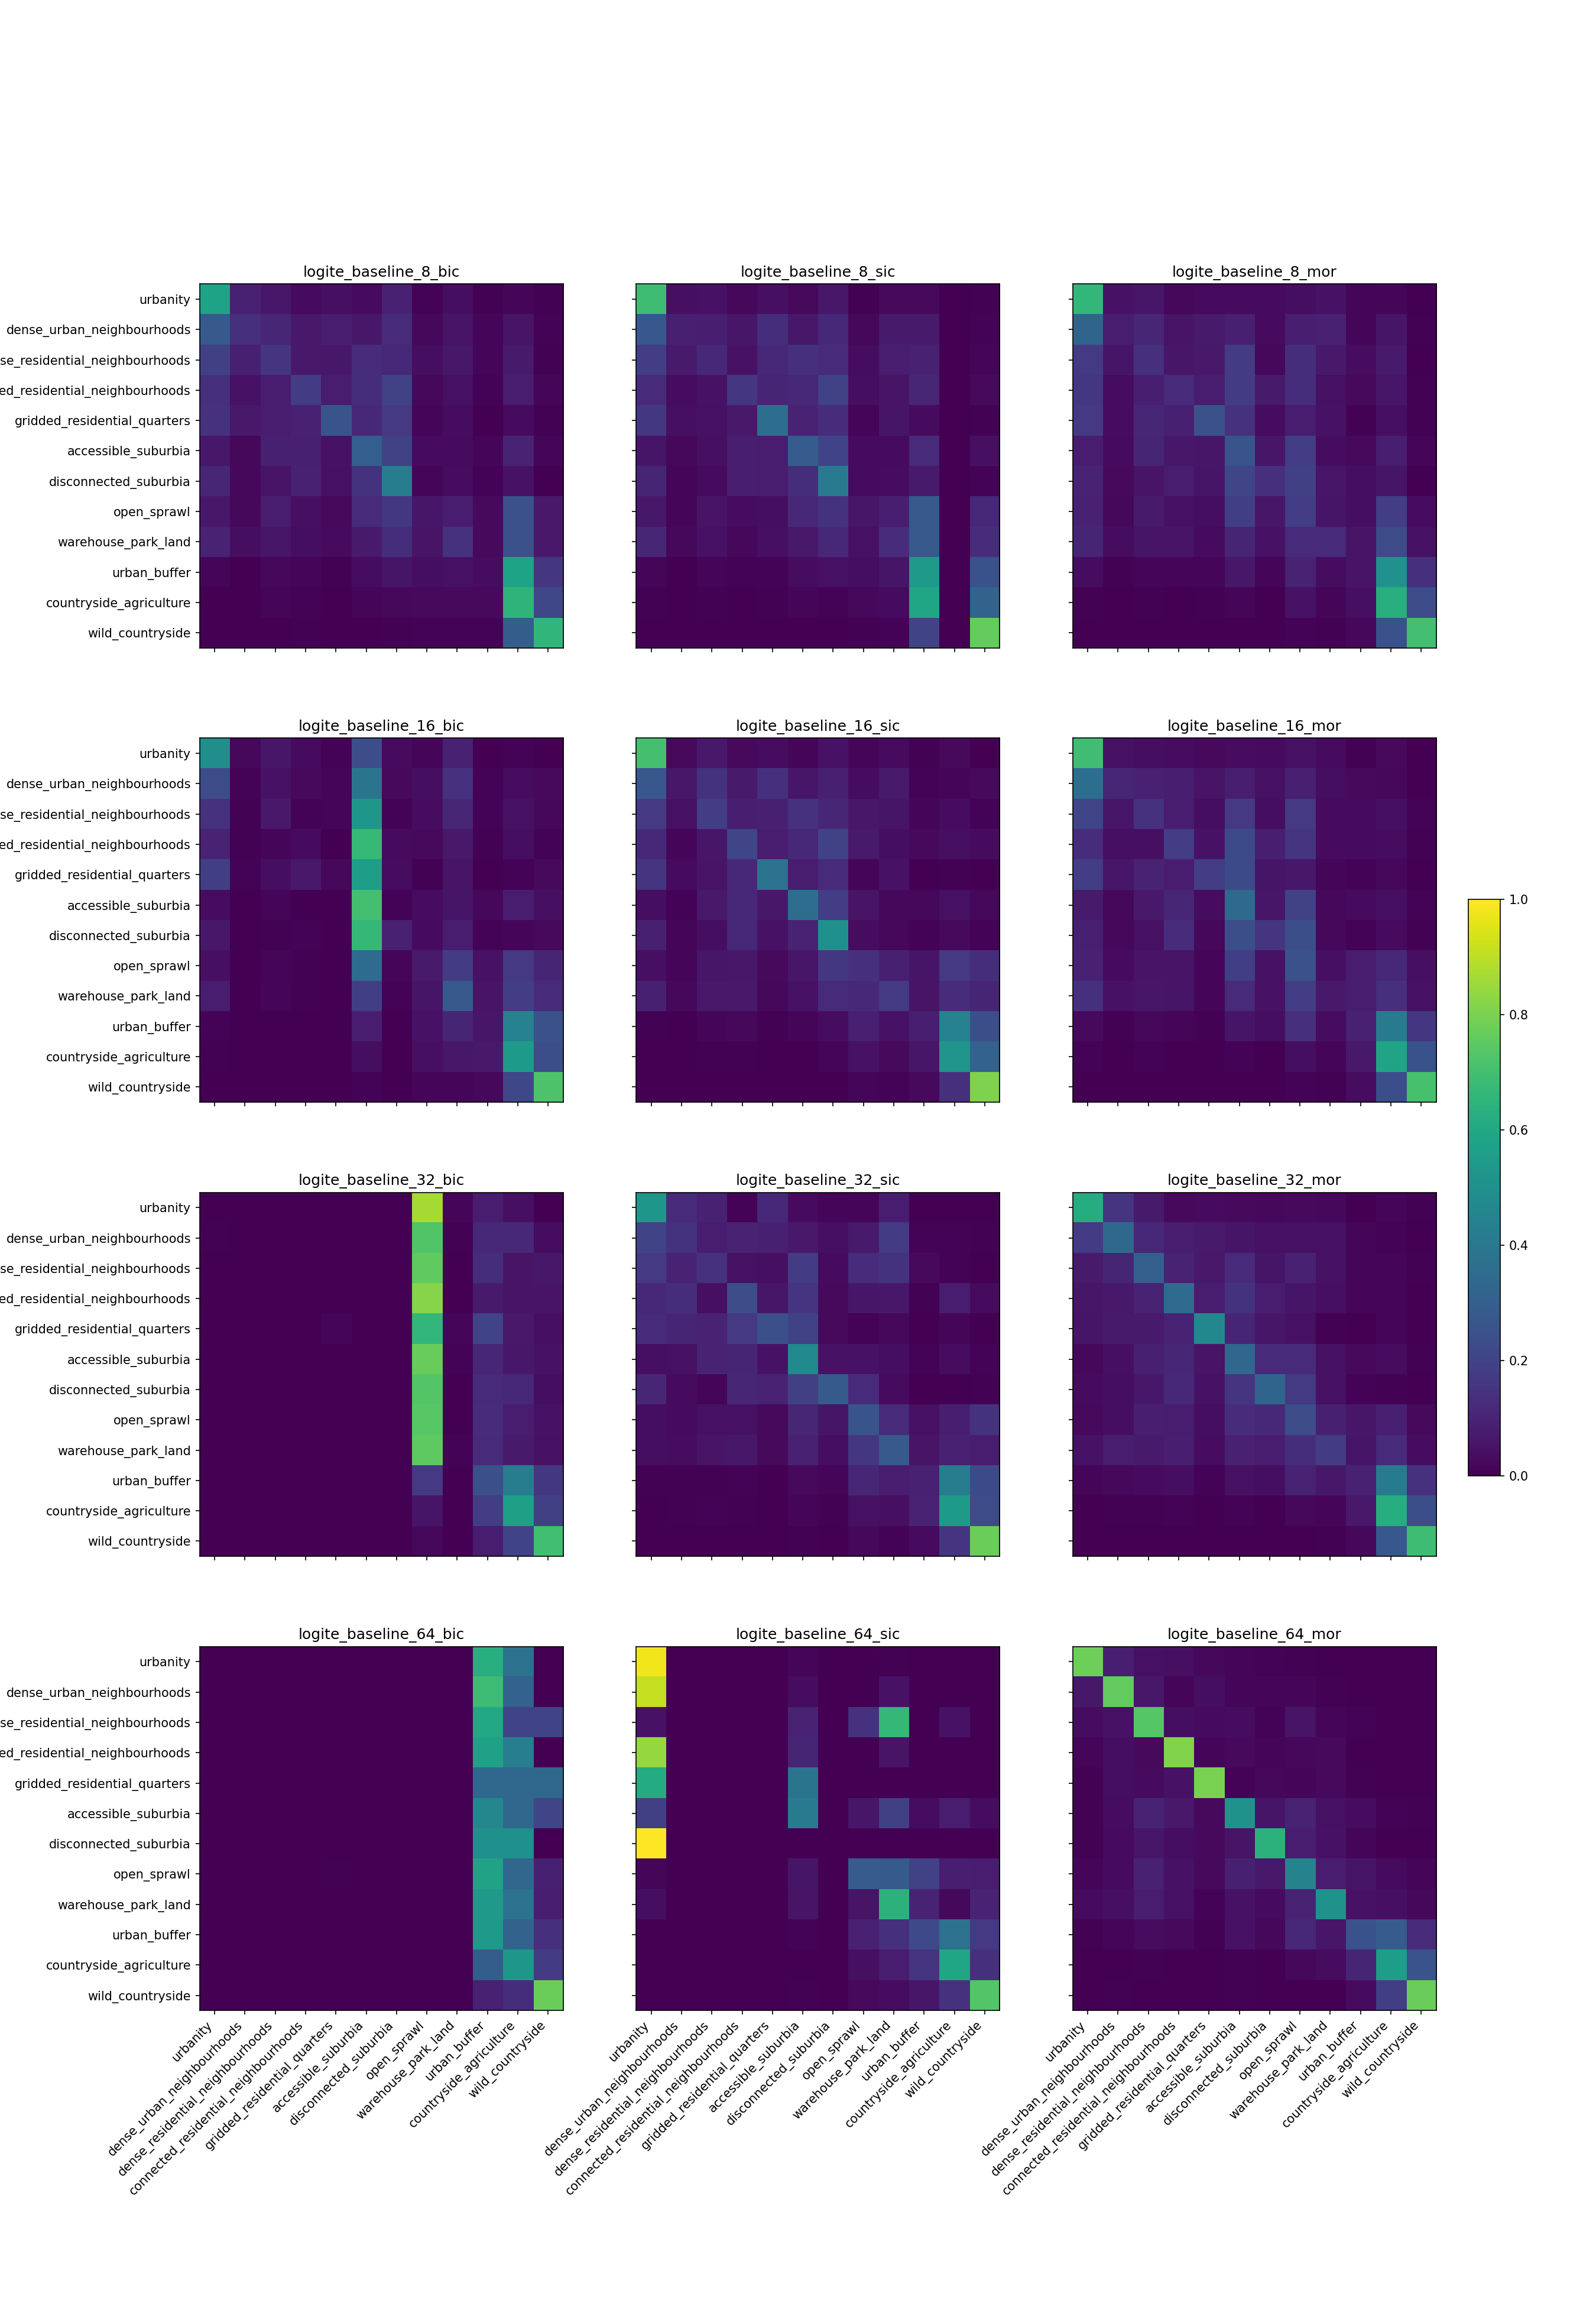
\includegraphics[width=.9\linewidth]{fig/logite_baseline_cm.png}
    \caption{\footnotesize Confusion matrices for individual models denoting
    the ability of each model in prediction of a correct label per each class
    using the logit ensemble baseline architecture.}
    \label{fig:logite_baseline_cm}
\end{figure}


\begin{figure}
    \centering
    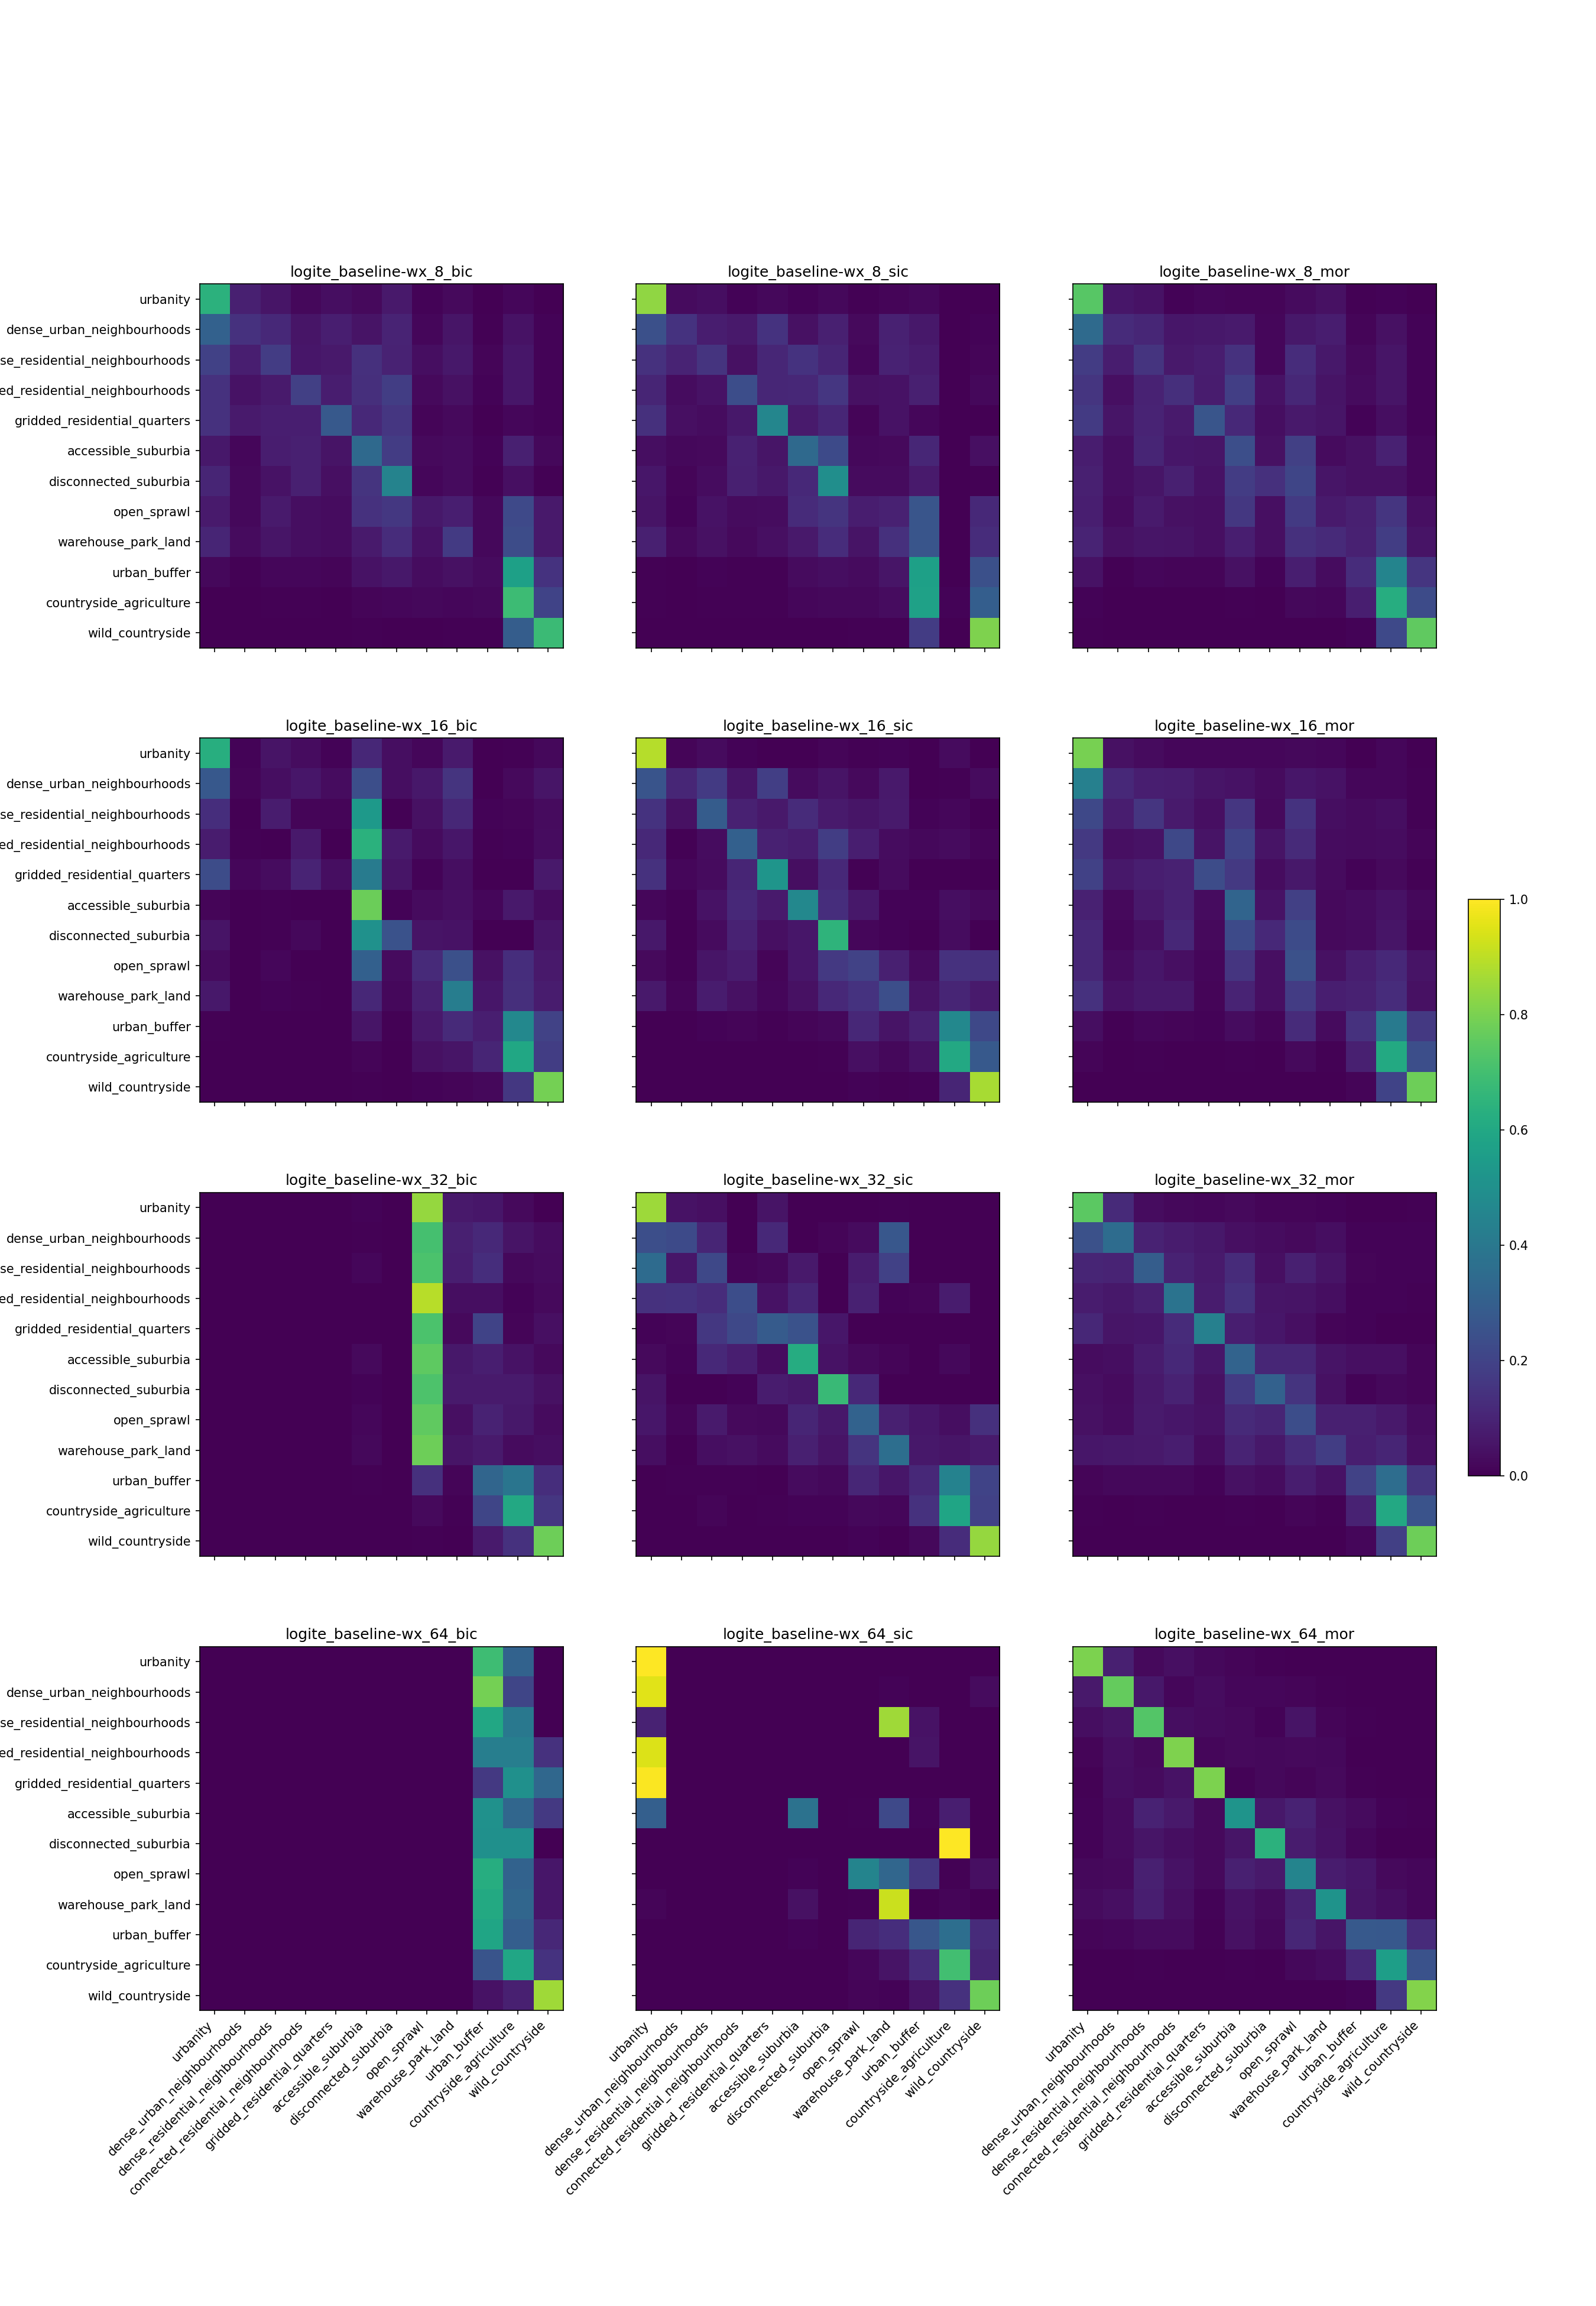
\includegraphics[width=.9\linewidth]{fig/logite_baseline-wx_cm.png}
    \caption{\footnotesize Confusion matrices for individual models denoting
    the ability of each model in prediction of a correct label per each class
    using the logit ensemble baseline-wx architecture.}
    \label{fig:logite_baseline-wx_cm}
\end{figure}


\begin{figure}
    \centering
    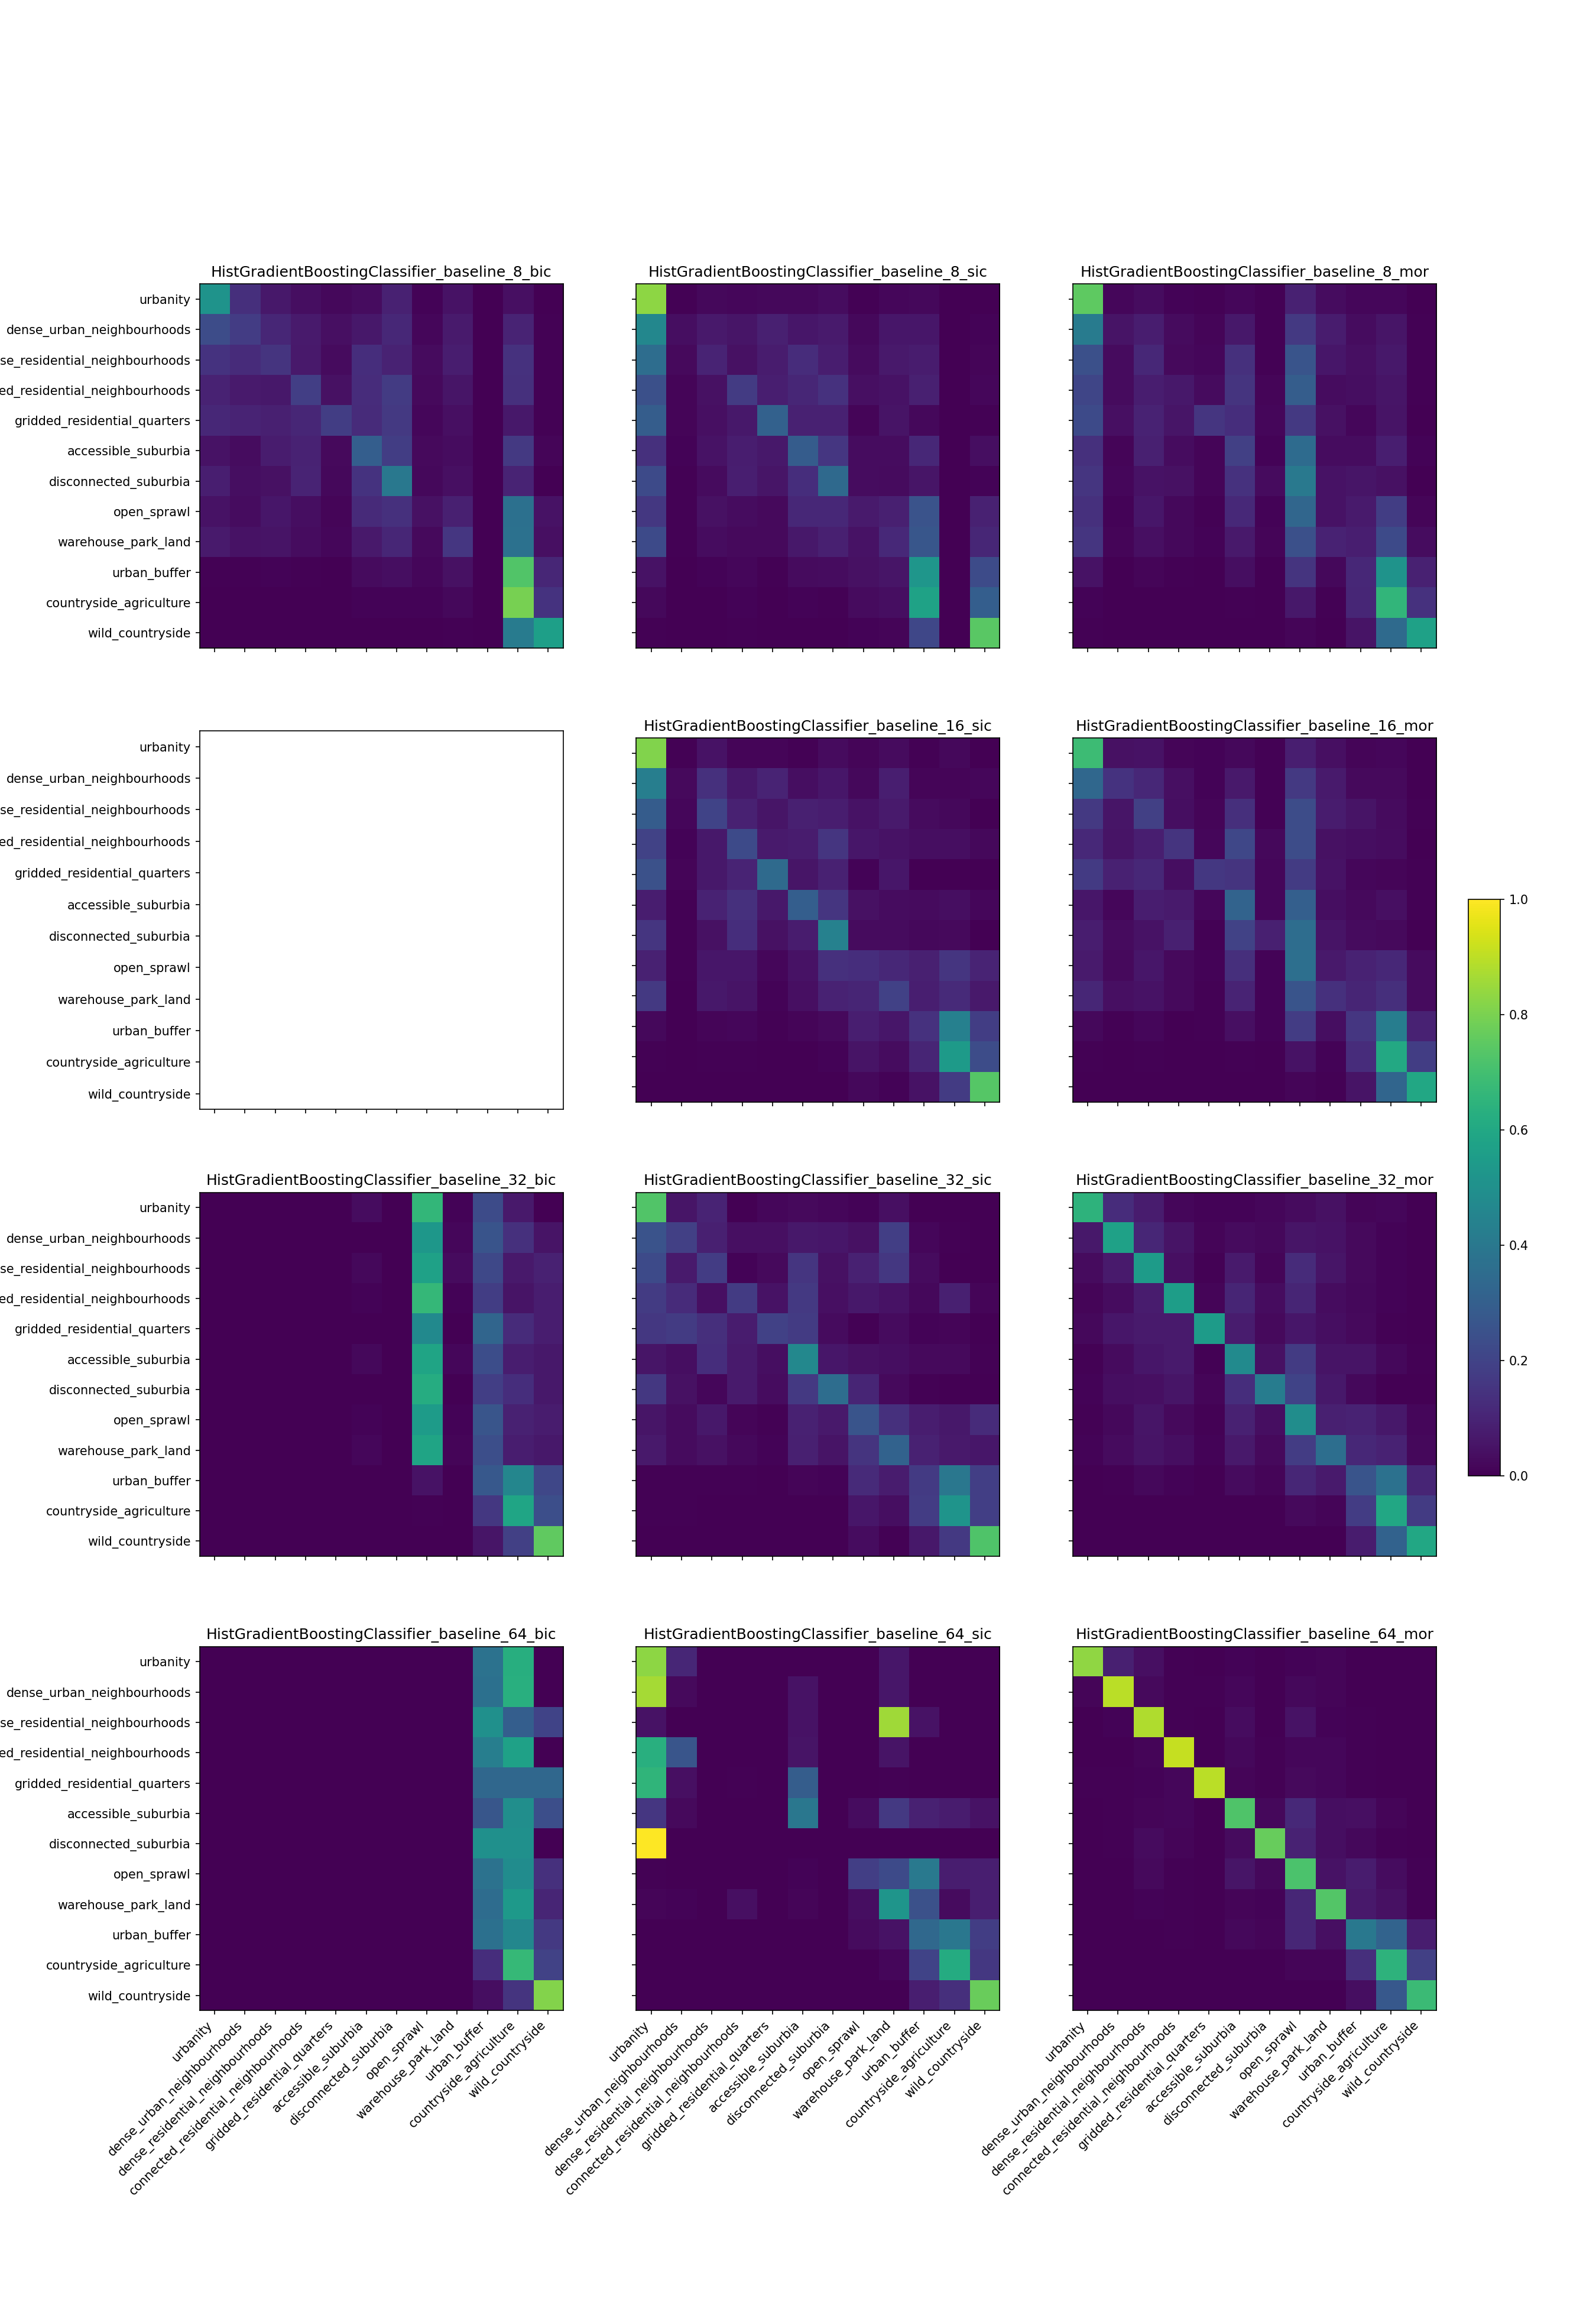
\includegraphics[width=.9\linewidth]{fig/HistGradientBoostingClassifier_baseline_cm.png}
    \caption{\footnotesize Confusion matrices for individual models denoting
    the ability of each model in prediction of a correct label per each class
    using the HGBC baseline architecture.}
    \label{fig:HistGradientBoostingClassifier_baseline_cm}
\end{figure}



\begin{figure}
    \centering
    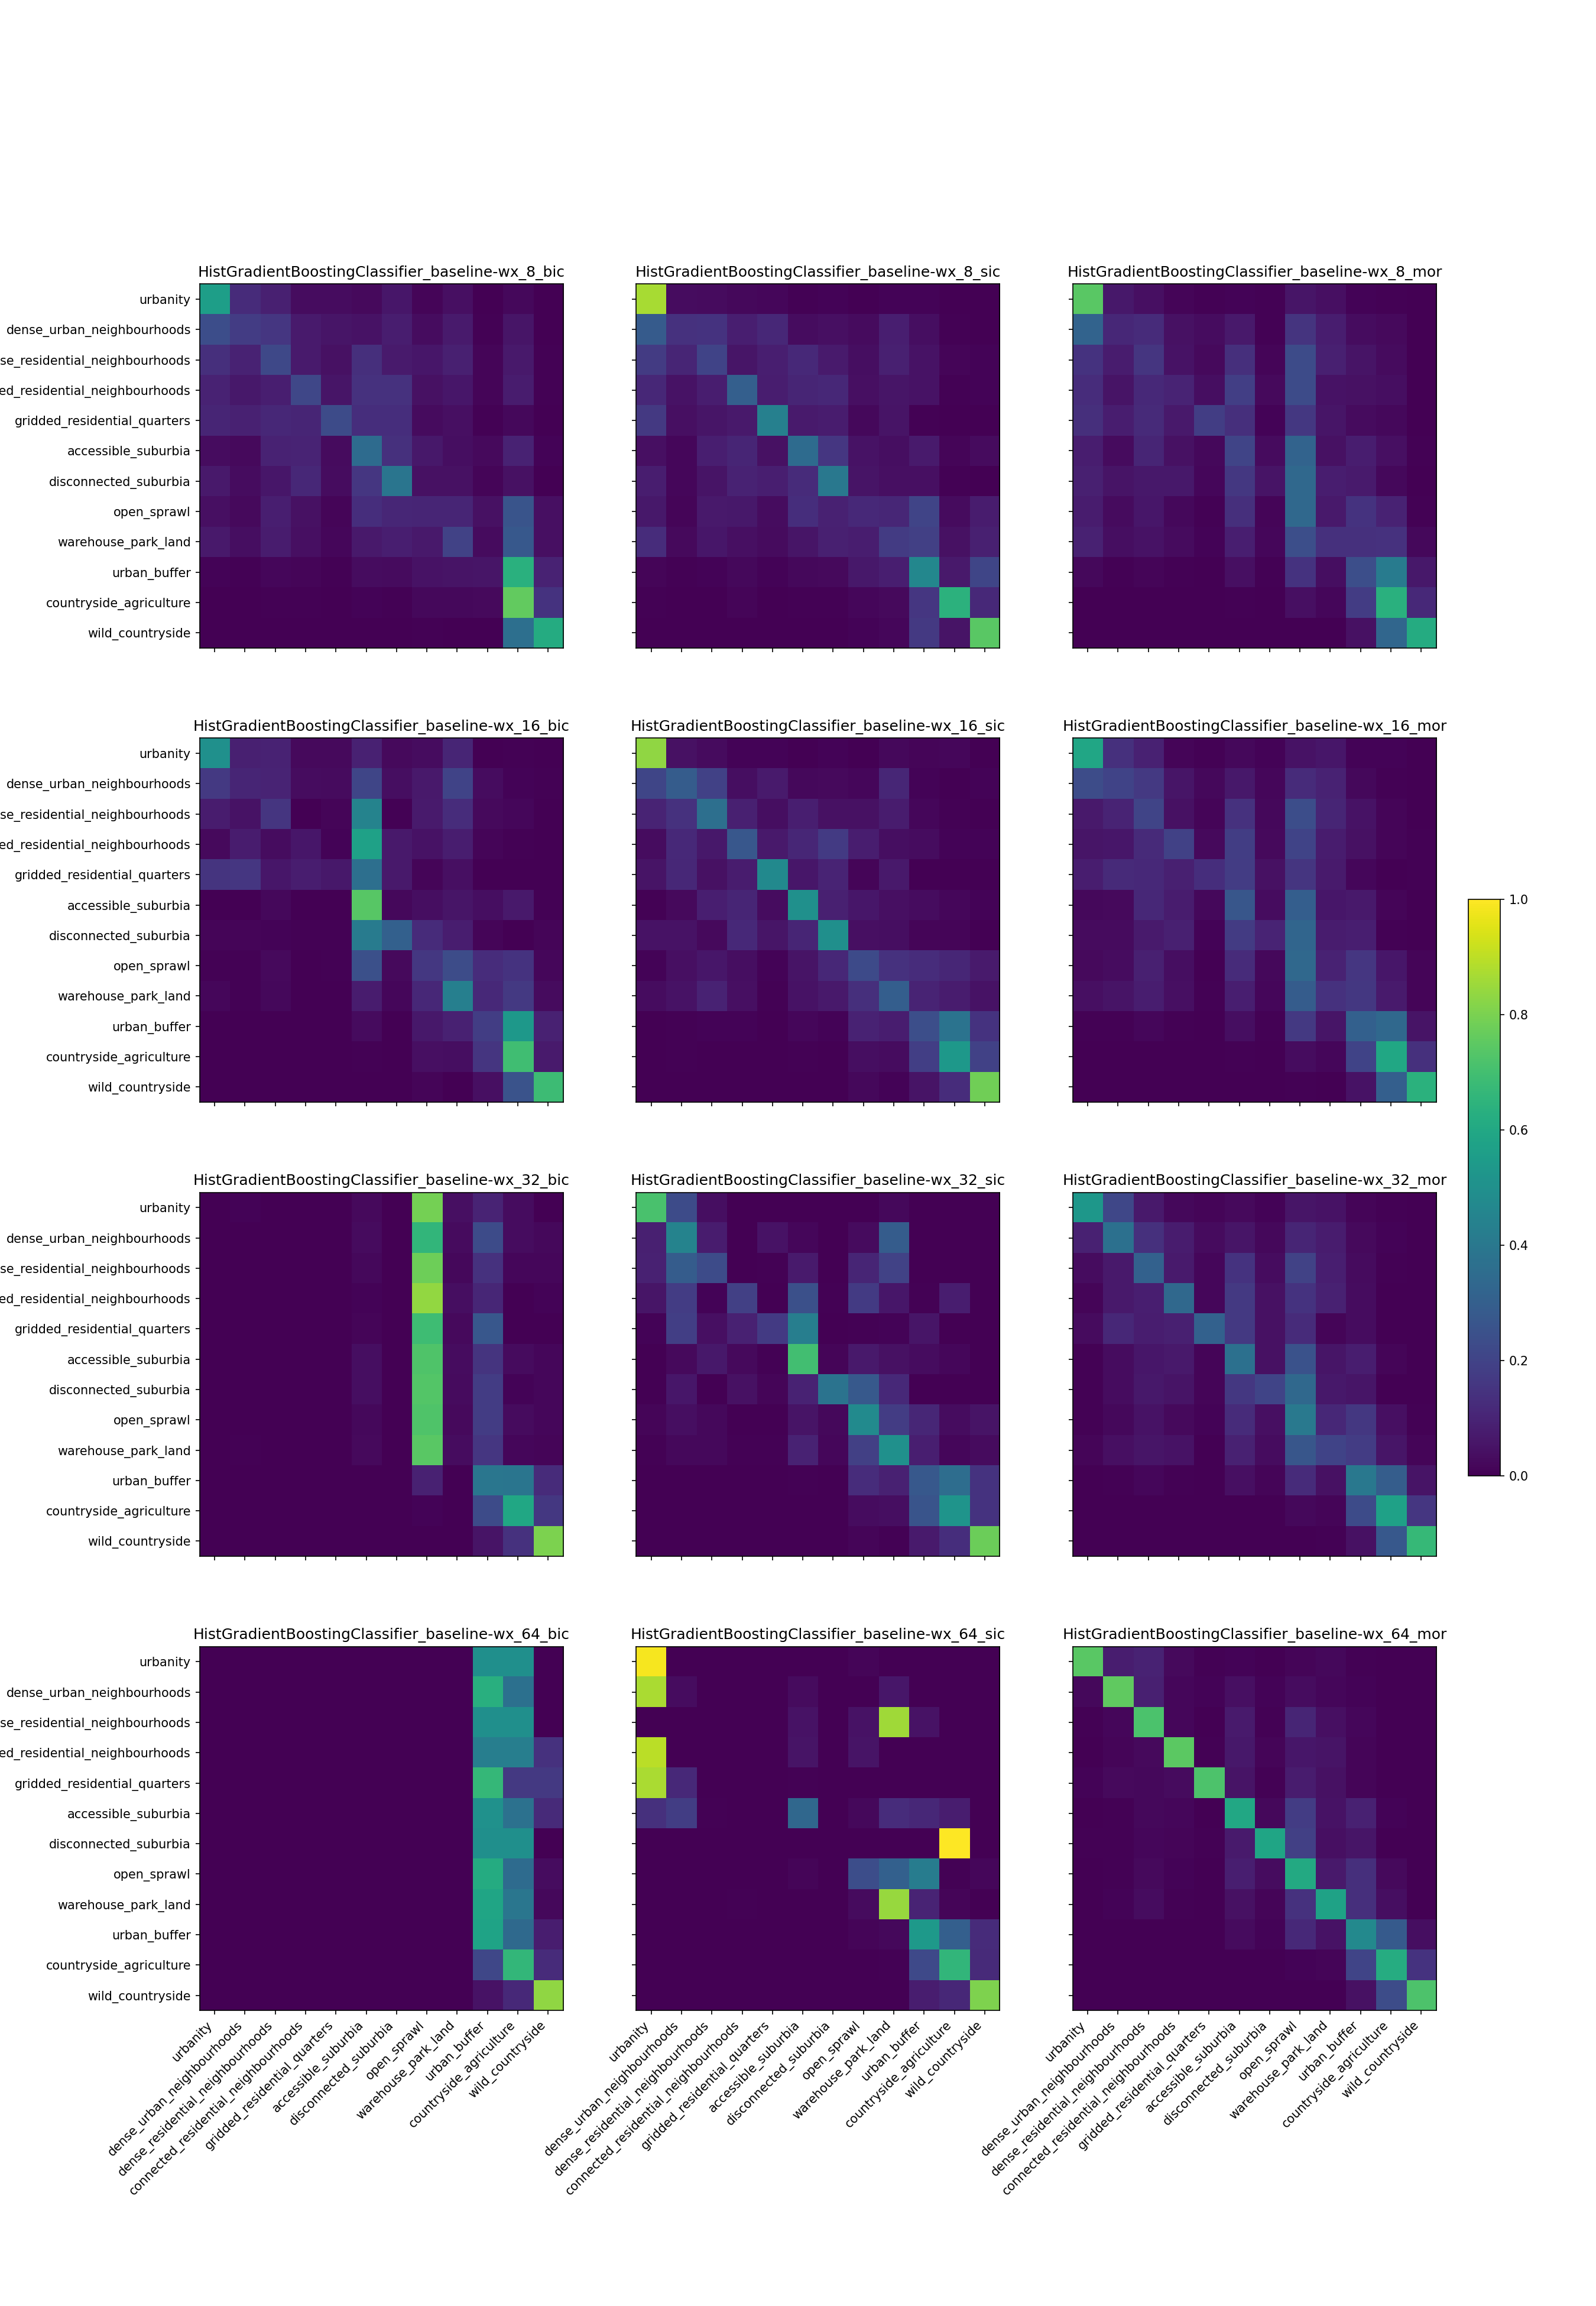
\includegraphics[width=.9\linewidth]{fig/HistGradientBoostingClassifier_baseline-wx_cm.png}
    \caption{\footnotesize Confusion matrices for individual models denoting
    the ability of each model in prediction of a correct label per each class
    using the HGBC baseline-wx architecture.}
    \label{fig:HistGradientBoostingClassifier_baseline-wx}
\end{figure}


\subsection{Fit of chips within signature types}

\begin{figure}
    \centering
    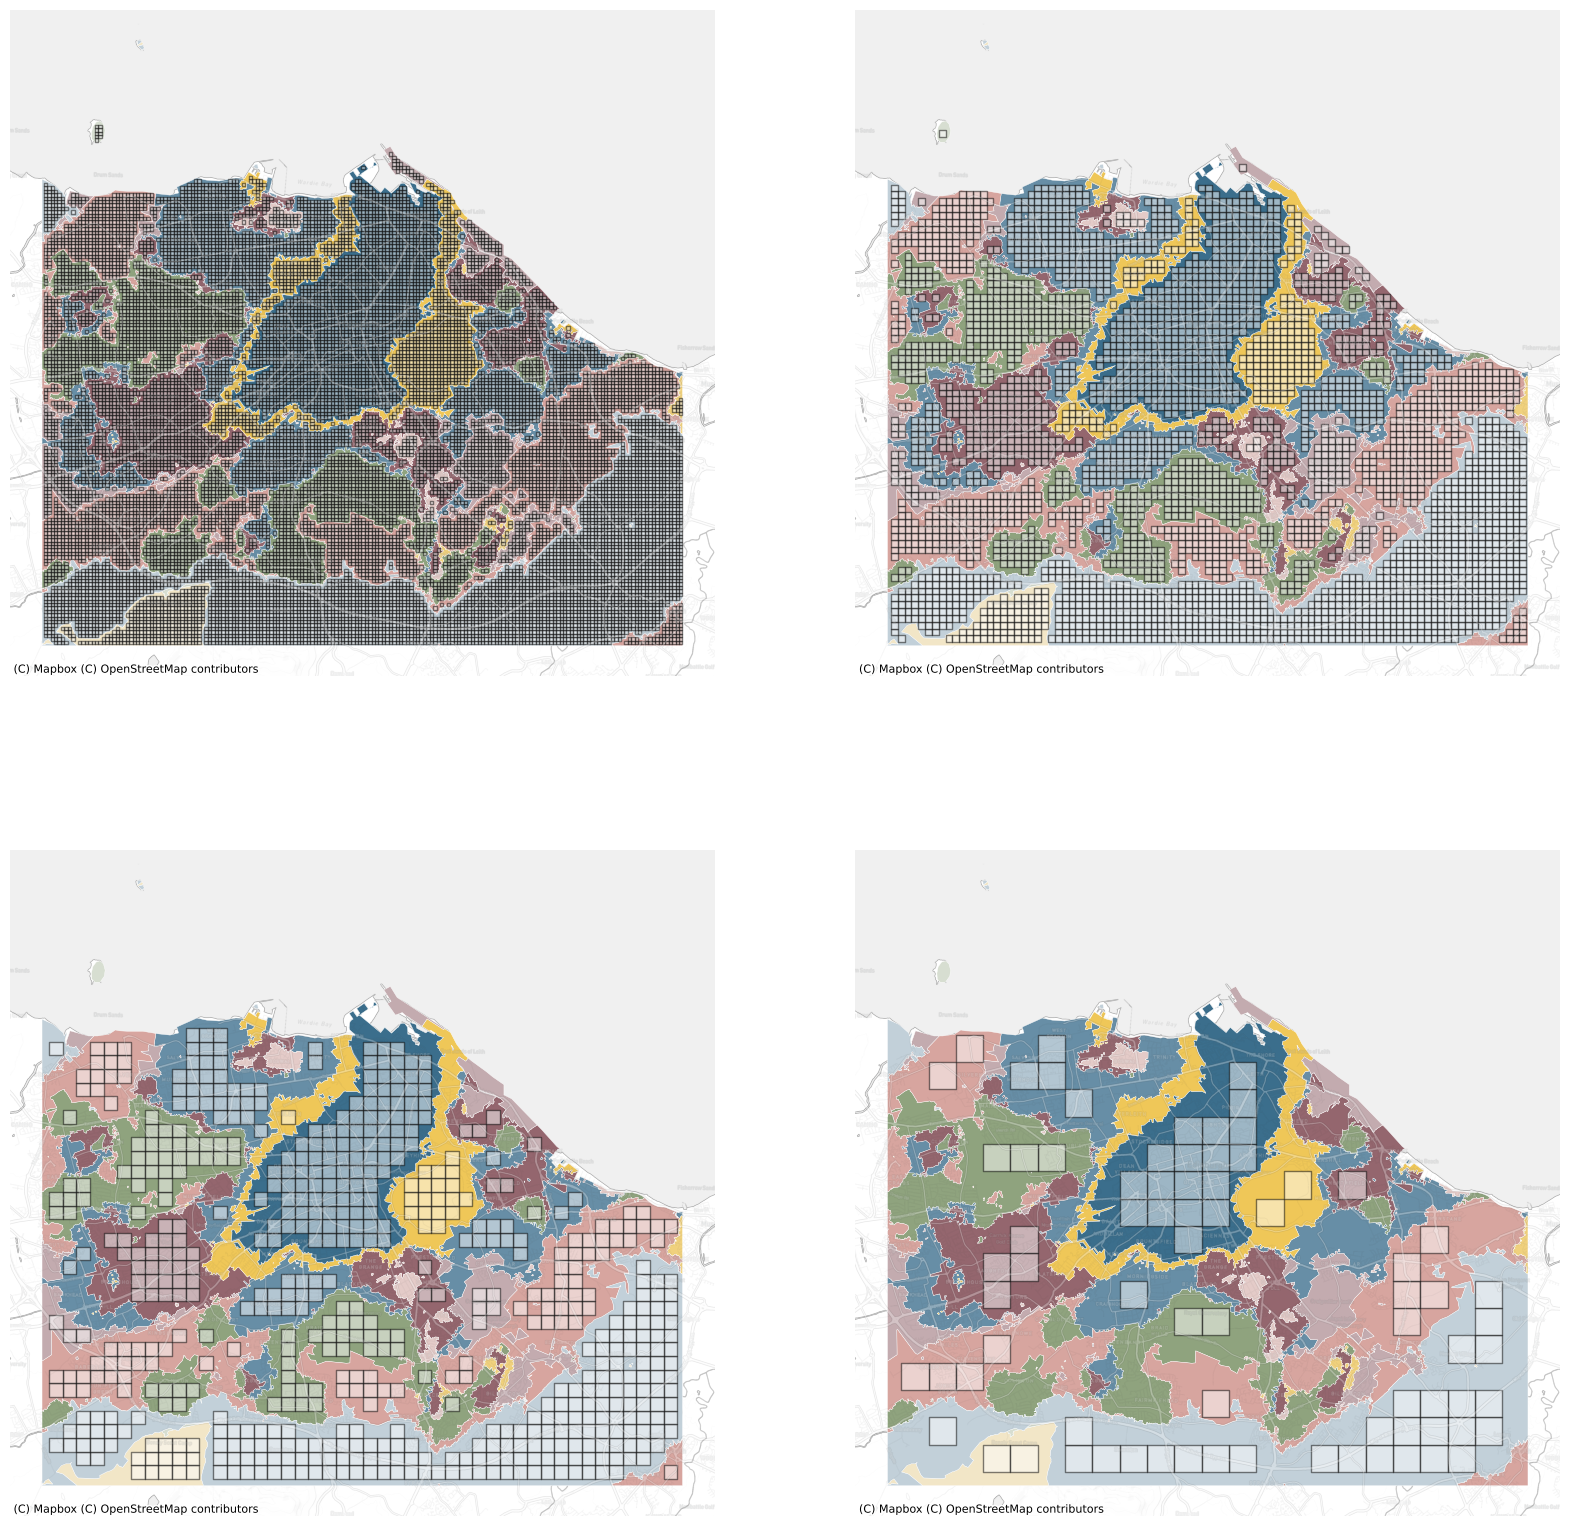
\includegraphics[width=0.8\linewidth]{fig/chip_fits.png}
    \caption{\footnotesize An illustration of the relationship between chip size and
    signature geometry in Edinburgh area. Subplots show all chips that represent a single
    class using 80 meters (top left), 160 m (top right), 320 m (bottom left) and 640 m (bottom right) chip sizes.}
    \label{fig:chip_fits}
\end{figure}

\pagebreak

\subsection{Chip counts}
\begin{table}
    \centering
\begin{tabular}{lrrr}
    \toprule
     & B.I.C. & S.I.C & M.O.R. \\
    \midrule
    8 & 534,729 & 1,099,439 & 135,264 \\
    16 & 331,459 & 1,087,827 & 126,016 \\
    32 & 179,261 & 901,538 & 112,196 \\
    64 & 132,619 & 373,131 & 94,960 \\
    \bottomrule
    \end{tabular}
\caption{\label{tab:chip_counts}\footnotesize Total number of chips (within all training, validation and secret sets) per chip size and architecture.}
\end{table}
